\section{Durchführung}
\label{sec:Durchführung}
In diesem Versuch werden alle untersuchten Schwing- und Schwebedauern für zwei unterschiedliche Pendellängen bestimmt. Dies kann durch unterschiedliche Aufhängungen der Masse am 
Pendel realisiert werden, da die angehängte Masse sehr viel Größer ist als die überstehende Masse des Metallstabes (siehe \autoref{fig:Aufbau1}).
Die Schwing- und Schwebedauern werden für verschiedene Arten von Schwingungen gemessen. Vorbereitent dazu wird zunächst überlegt, ob es sich bei diesem Versuch um eine 
harmonische Schwingung handelt. Eine harmonische Schwingung muss durch  Sinus- und Kosinusfunktionen beschrieben werden können und es muss ein lineares Kraftgesetzt gelten.
Außerdem muss die Energie erhalten sein. Die ersten beiden Bedingungen gelten für ein Pendel, wie es im Versuch genutzt wird. Aufgrund der kurzen Messdauern kann annähernde 
Energieerhaltung angenommen werden. Um nun die Gleichungen aus \autoref{sec:Theorie} nutzen zu können, dürfen bei der Durchführung lediglich kleine Auslenkungen der Pendel 
verwendet werden, also solche, bei denen die Kleinwinkelnäherung noch möglichst genau gilt. Dies ist bis zu einem Auslenkwinkel von circa $5\textdegree$ gegeben. 


Für diesen Versuch benötigt man zwei identische Pendel (siehe \autoref{fig:Aufbau1}), welche durch eine Feder gekoppelt werden können (siehe \autoref{fig:Aufbau2}).
\begin{figure}
    \centering
    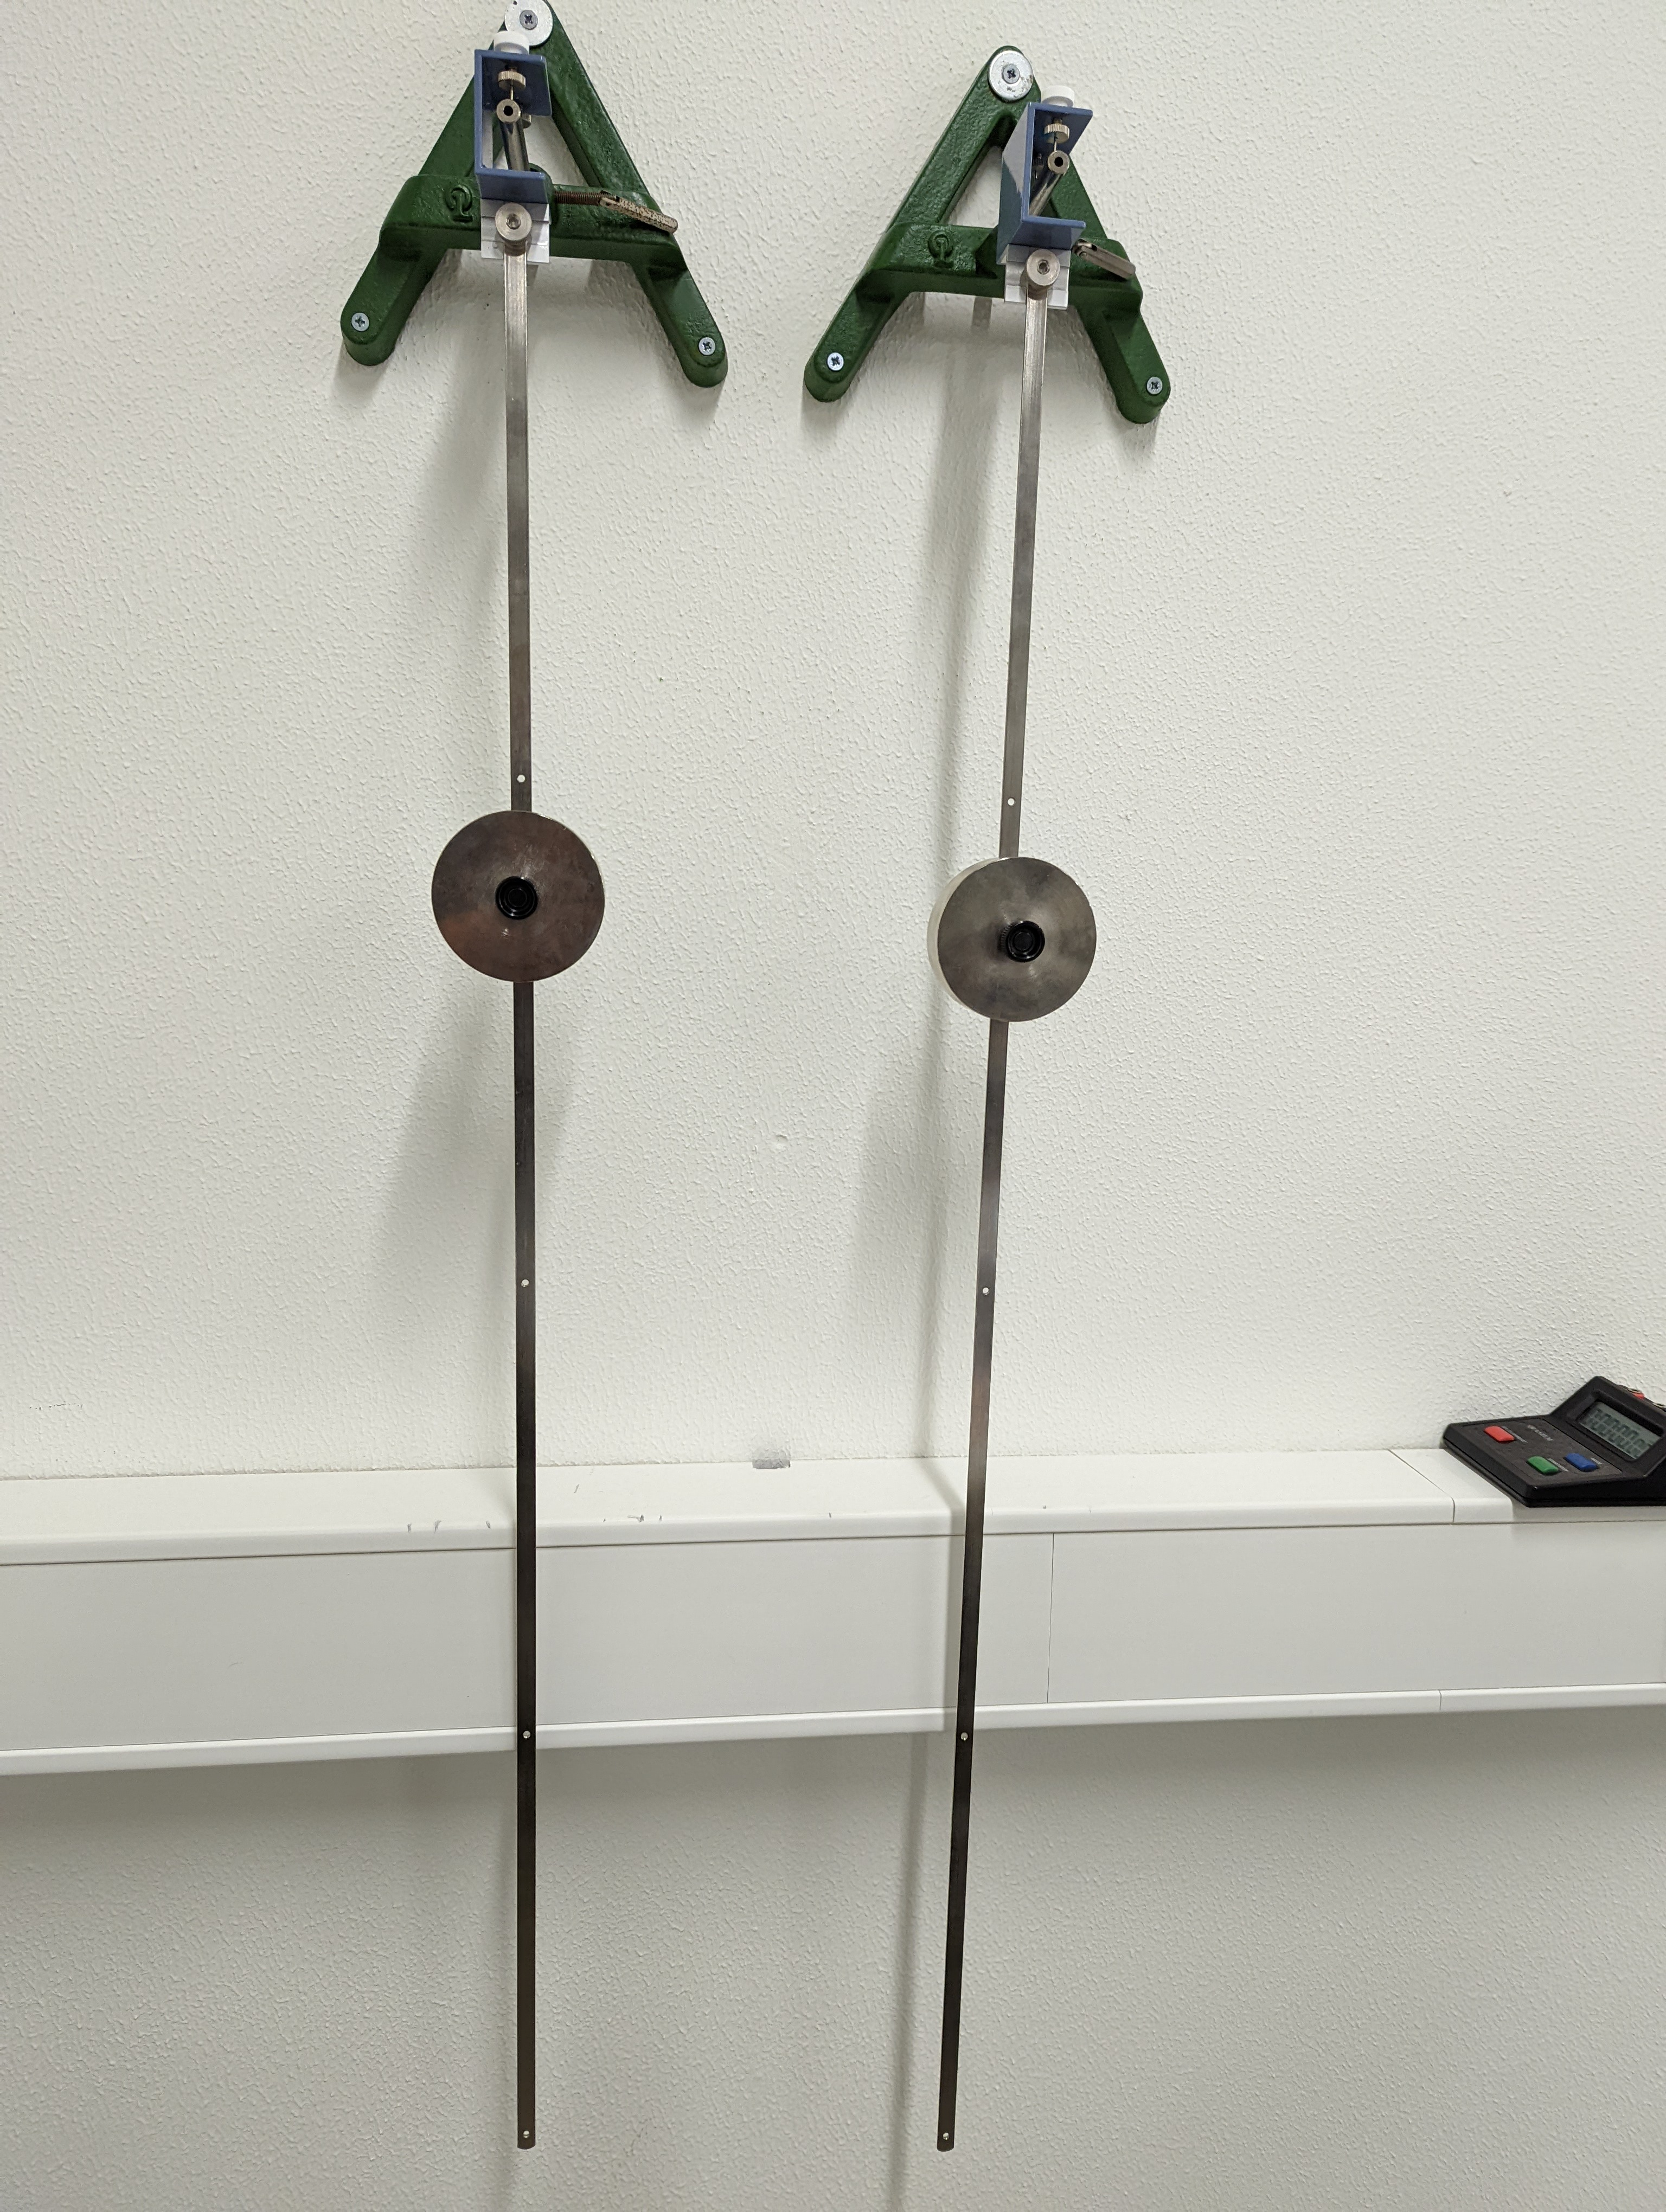
\includegraphics[width=0.4\textwidth]{content/Einzelpendel.jpg}
	\caption{Aufbau des Versuchs: Zwei Stabpendel mit höhenverstellbaren Massen.}
	\label{fig:Aufbau1}
\end{figure}
Zuerst wird die Schwingungsdauer eines einfachen Pendels bestimmt. Dazu werden fünf Schwingungsdauern gemessen um den Fehler der Zeitmessung möglichst klein zu halten.
Dies wird zehn mal an beiden Pendeln durchgeführt, um auch die möglichen Unterschiede der beiden Einzelpendel zueinander gemessen zu haben. 


Anschließend wird die Kopplungsfeder an die Pendel angebracht, wie es in \autoref{fig:Aufbau2} zu sehen ist. 
\begin{figure}
    \centering
    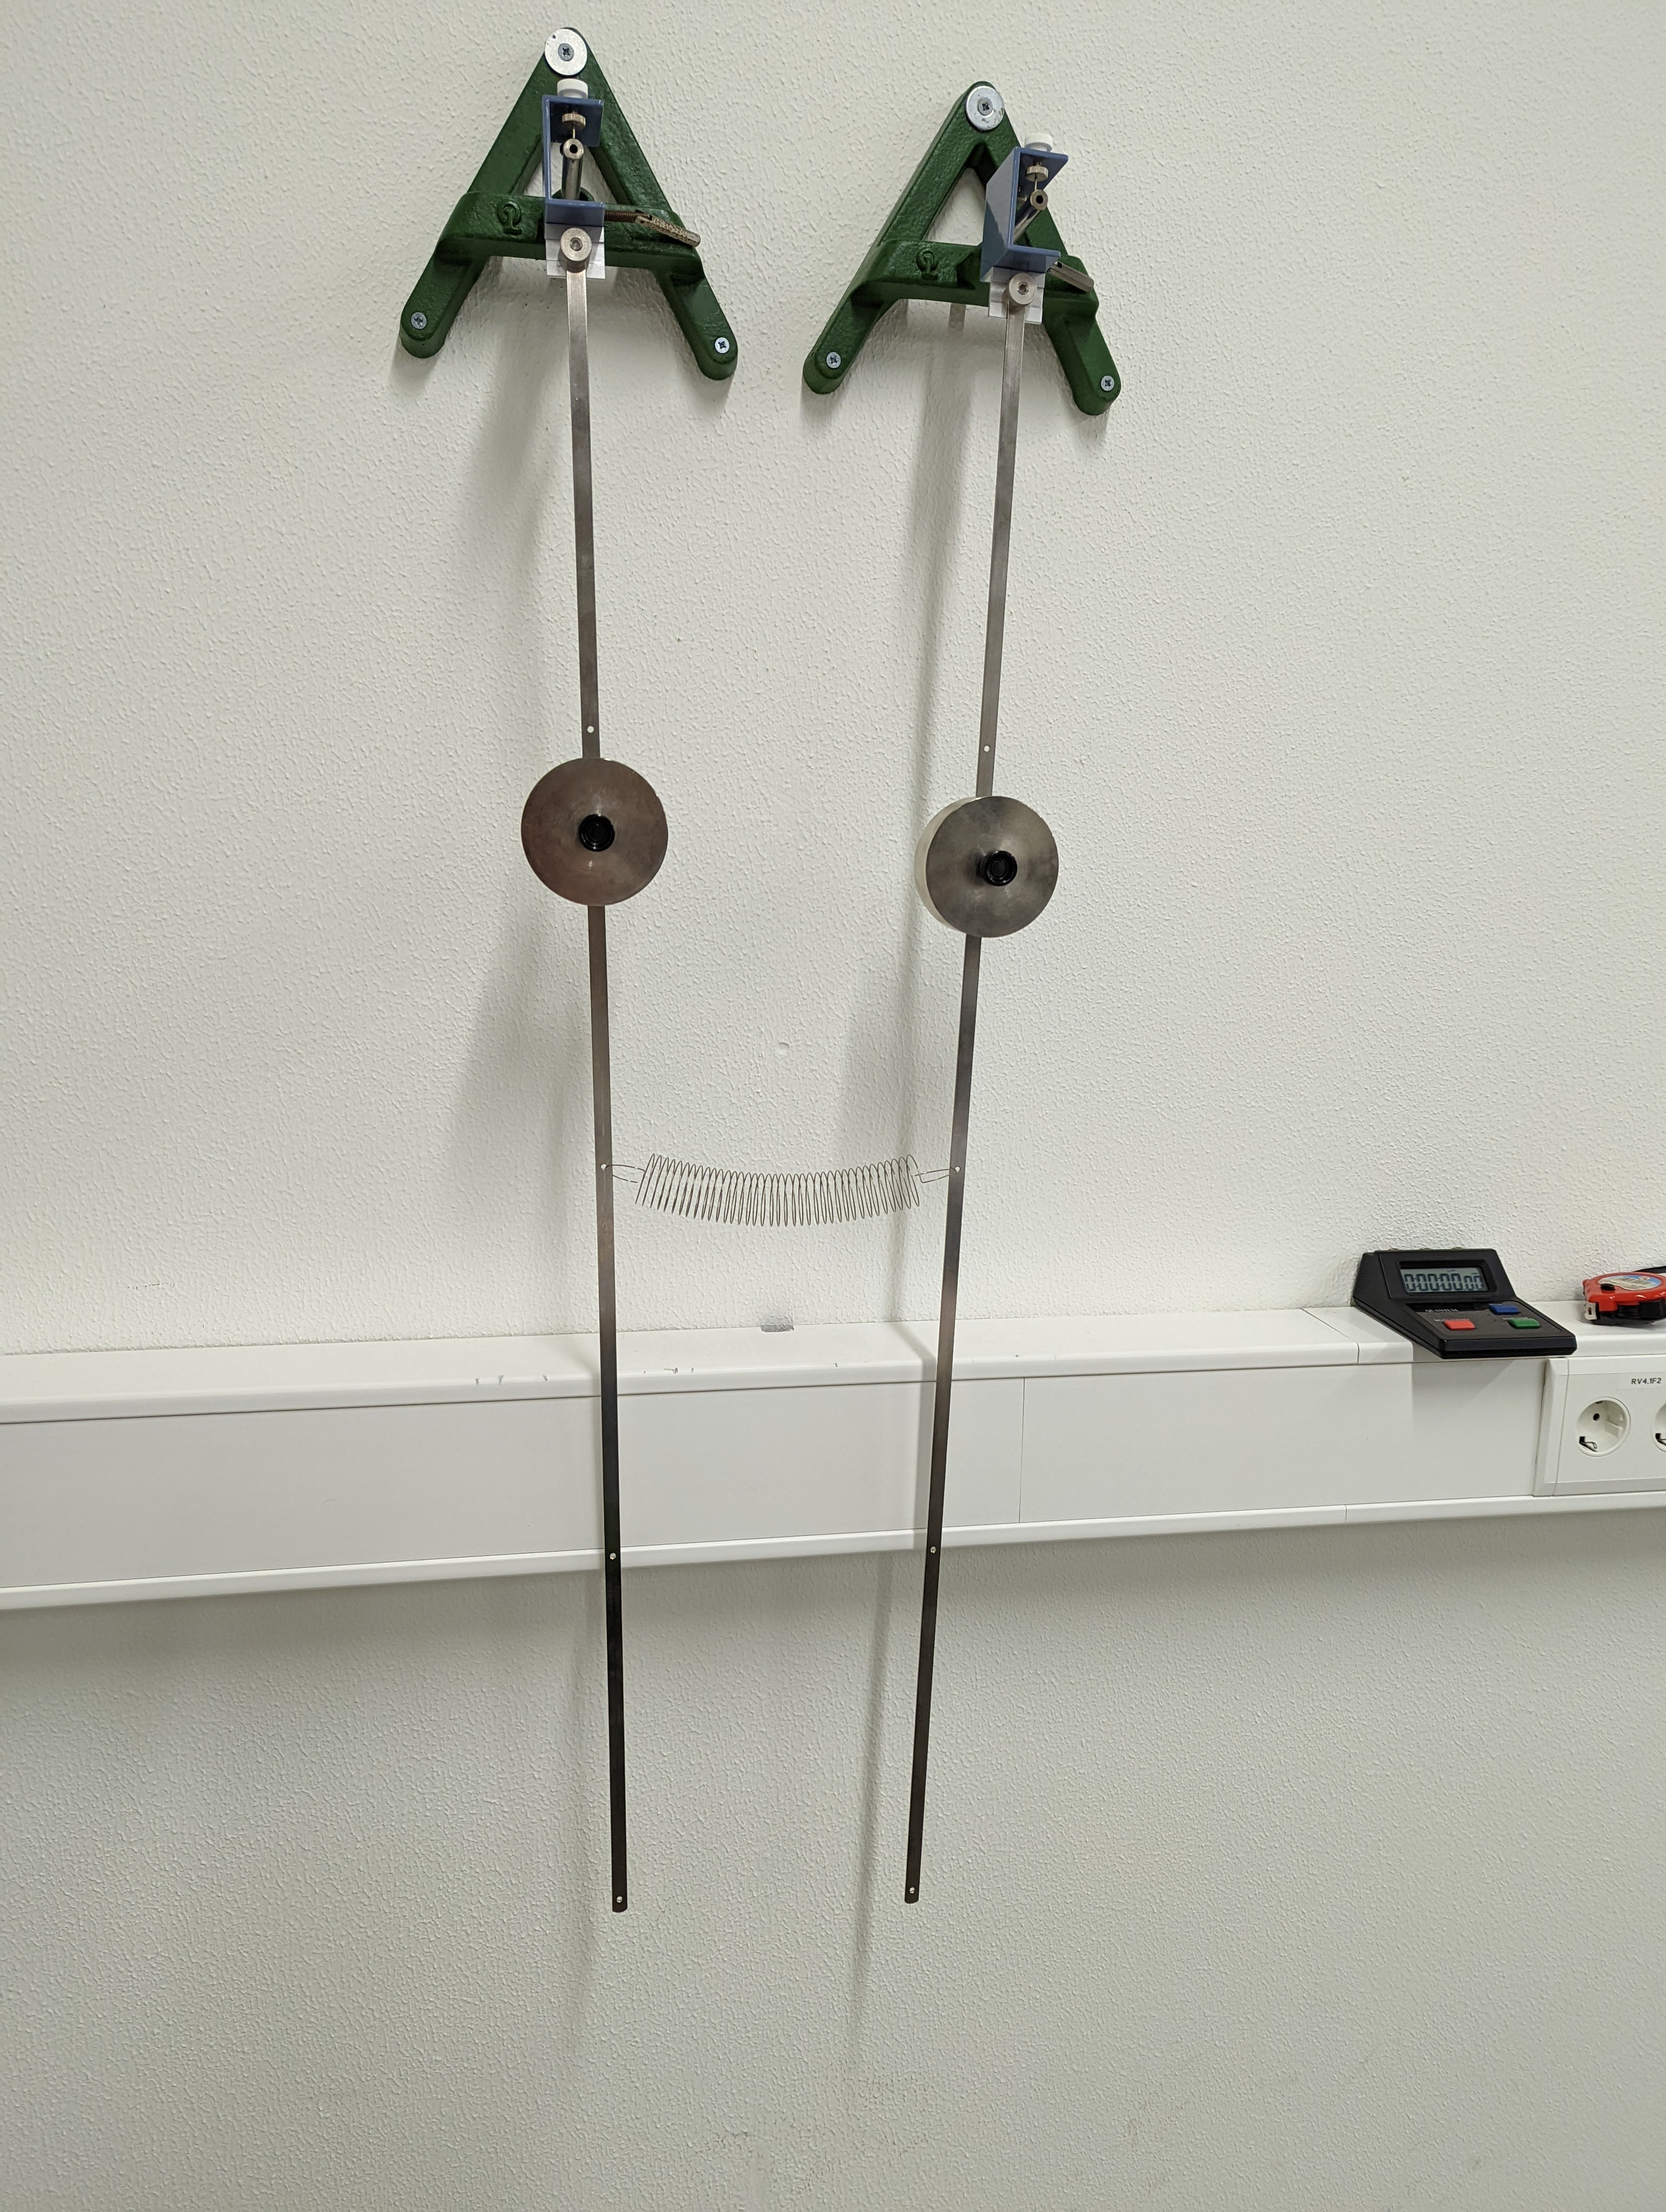
\includegraphics[width=0.4\textwidth]{content/Gekoppelt.jpg}
	\caption{Stabpendel mit Kopplungsfeder.}
	\label{fig:Aufbau2}
\end{figure}
Zuerst wird eine gleichsinnige Schwingung der gekoppelten Pendel untersucht. Dazu werden die Pendel, wie in \autoref{fig:Gleichsinnig} zu sehen ist, um den gleichen Winkel ausgelenkt.
Es werden erneut zehn Messungen durchgeführt, bei denen je fünf Schwingungsperioden gemessen werden.

Danach wird die gegensinnige Schwingung untersucht. Die Pendel werden gemäß \autoref{fig:Gegensinnig} ausgelenkt. Wie zuvor werden zehn Messwerte für die Dauer von je fünf Perioden der
Schwingung gemessen.


Zuletzt wird die gekoppelte Schwingung beziehungsweise der Schwebungsfall untersucht. Eines der Pendel soll sich in Ruhelage befinden während das Andere ausgelenkt wird. 
\autoref{fig:Schwebung} stellt die beschrieben Auslenkung dar. Hier wird die Schwebungssdauer von einer Ruhelage eines Pendels bis zu seiner nächsten bestimmt. Dabei muss sehr
genau beobachtet werden wann die Ruhelage eintritt, da kurz vor der Ruhelage noch sehr kleine Schwingungen ausgeübt werden. Zu dieser Messung reicht es, eine Periode der Schwebung
zu messen, da diese ausreichend lang ist. Zusätzlich wird die Schwingungsdauer eines Pendels gemessen. Diese ist beim Schwebungsfall bei einem der Pendel zwisches dessen Ruhelagen zu messen. Je nach länge 
des Pendel können hier nur 3-5 Schwingungsdauer gemessen werden, da sich das Pendel nach wenigen Schwingungen wieder in Ruhelage begibt. Es sollen ebenfalls 10 Messungen der Schwing- und Schwebedauern
durchgeführt werden. 